
%% bare_conf.tex
%% V1.4a
%% 2014/09/17
%% by Michael Shell
%% See:
%% http://www.michaelshell.org/
%% for current contact information.
%%
%% This is a skeleton file demonstrating the use of IEEEtran.cls
%% (requires IEEEtran.cls version 1.8a or later) with an IEEE
%% conference paper.
%%
%% Support sites:
%% http://www.michaelshell.org/tex/ieeetran/
%% http://www.ctan.org/tex-archive/macros/latex/contrib/IEEEtran/
%% and
%% http://www.ieee.org/

%%*************************************************************************
%% Legal Notice:
%% This code is offered as-is without any warranty either expressed or
%% implied; without even the implied warranty of MERCHANTABILITY or
%% FITNESS FOR A PARTICULAR PURPOSE! 
%% User assumes all risk.
%% In no event shall IEEE or any contributor to this code be liable for
%% any damages or losses, including, but not limited to, incidental,
%% consequential, or any other damages, resulting from the use or misuse
%% of any information contained here.
%%
%% All comments are the opinions of their respective authors and are not
%% necessarily endorsed by the IEEE.
%%
%% This work is distributed under the LaTeX Project Public License (LPPL)
%% ( http://www.latex-project.org/ ) version 1.3, and may be freely used,
%% distributed and modified. A copy of the LPPL, version 1.3, is included
%% in the base LaTeX documentation of all distributions of LaTeX released
%% 2003/12/01 or later.
%% Retain all contribution notices and credits.
%% ** Modified files should be clearly indicated as such, including  **
%% ** renaming them and changing author support contact information. **
%%
%% File list of work: IEEEtran.cls, IEEEtran_HOWTO.pdf, bare_adv.tex,
%%                    bare_conf.tex, bare_jrnl.tex, bare_conf_compsoc.tex,
%%                    bare_jrnl_compsoc.tex, bare_jrnl_transmag.tex
%%*************************************************************************


% *** Authors should verify (and, if needed, correct) their LaTeX system  ***
% *** with the testflow diagnostic prior to trusting their LaTeX platform ***
% *** with production work. IEEE's font choices and paper sizes can       ***
% *** trigger bugs that do not appear when using other class files.       ***                          ***
% The testflow support page is at:
% http://www.michaelshell.org/tex/testflow/



\documentclass[conference]{IEEEtran}
% Some Computer Society conferences also require the compsoc mode option,
% but others use the standard conference format.
%
% If IEEEtran.cls has not been installed into the LaTeX system files,
% manually specify the path to it like:
% \documentclass[conference]{../sty/IEEEtran}

\usepackage{amsmath}

% Some very useful LaTeX packages include:
% (uncomment the ones you want to load)
% ---
% PACOTES
% ---
\usepackage[brazil]{babel}		% Idioma do documento
\usepackage{color}			% Controle das cores
\usepackage[T1]{fontenc}		% Selecao de codigos de fonte.
\usepackage{graphicx}			% Inclusão de gráficos
\usepackage[utf8]{inputenc}		% Codificacao do documento (conversão automática dos acentos)
\usepackage[noadjust]{cite}
\usepackage{txfonts}			% Fontes virtuais
\usepackage{listings}
\usepackage{adjustbox}
\usepackage{tabularx}
\usepackage{multirow}
\usepackage{multicol}
\usepackage{colortbl}
\usepackage{caption}
\usepackage{pgf}
\usepackage{tikz}
\usetikzlibrary{arrows,shapes,automata,positioning}


\usepackage{filecontents}
\begin{filecontents*}{references.bib}
	@IEEEtranBSTCTL{IEEEexample:BSTcontrol,
		CTLdash_repeated_names = "no",
	}
	
	@article{Zhang05,
		author = "Author1 and Author2",
		title = "{The title}",
		booktitle = {ACM},
		year = {2005},
		volume = {3},
		issue = {2},
		pages = {363-387},
	}
\end{filecontents*}

% correct bad hyphenation here
\hyphenation{op-tical net-works semi-conduc-tor}

\begin{document}
%
% paper title
% Titles are generally capitalized except for words such as a, an, and, as,
% at, but, by, for, in, nor, of, on, or, the, to and up, which are usually
% not capitalized unless they are the first or last word of the title.
% Linebreaks \\ can be used within to get better formatting as desired.
% Do not put math or special symbols in the title.
\title{Estudo e modelagem do controle supervisório de um sistema distribuído de tempo real crítico para veículos autônomos terrestres}

% author names and affiliations
% use a multiple column layout for up to three different
% affiliations
\author{
	\IEEEauthorblockN{Carlos F. de P. Perché}
	\IEEEauthorblockA{Faculdade de Engenharia Mecânica\\
	Faculdade Estadual de Campinas\\
	Campinas, SP, Brasil 13083--770\\
	Email: cfpperche@gmail.com}
}

% make the title area
\maketitle

% As a general rule, do not put math, special symbols or citations
% in the abstract
\begin{abstract}
The abstract goes here.
\end{abstract}

% no keywords

\IEEEpeerreviewmaketitle
% -------------------- NEW SECTION -------------------- 
% -------------------- NEW SECTION -------------------- 
% -------------------- NEW SECTION -------------------- 
\section{Introduction}\label{sec:introduction}
\subsection{Objectives}\label{subsec:objectives}
\subsection{Requirements}\label{subsec:requirements}
% -------------------- NEW SECTION -------------------- 
% -------------------- NEW SECTION -------------------- 
% -------------------- NEW SECTION -------------------- 
\section{Architecture Concepts}\label{sec:architec_concepts}
\subsection{Unmanned Vehicles}\label{subsec:unmanned_vehicles}
\subsection{Critical Systems}\label{subsec:unmaned_vehicles}
\subsection{Real-Time Systems}\label{subsec:real_time_systems}
\subsection{Robot Systems}\label{subsec:robot_systems}
\subsection{Automata for modeling real-time systems}\label{subsec:automata_systems}

% -------------------- NEW SECTION -------------------- 
% -------------------- NEW SECTION -------------------- 
% -------------------- NEW SECTION -------------------- 
\section{Architecture Components}\label{sec:architec_components}
\subsection{Linux}\label{subsec:linux}
\subsection{Xenomai}\label{subsec:xenomai}
\subsection{RTnet}\label{subsec:rtnet}
\subsection{ROS}\label{subsec:ros}
\subsection{OROCOS}\label{subsec:orocos}
% -------------------- NEW SECTION -------------------- 
% -------------------- NEW SECTION -------------------- 
% -------------------- NEW SECTION -------------------- 

\section{Proposed Architecture}\label{sec:proposed_architec}
\subsection{Operational Modes}\label{subsec:operational_modes}
\subsection{Modules and Components}\label{subsec:modules_components}
\subsection{States and Transitions for Supervisory Control}\label{subsec:states_transitions}
\subsection{Implementation}\label{subsec:implementation}
\subsubsection{General Description of Module Behavior}\label{subsec:module_behavior}
\subsubsection{Software Processes}\label{subsec:software_processes}

% uformal_synthesis
\subsubsection{Implication on Formal Synthesis}\label{subsec:formal_synthesis}

Após o modelamento que determina o comportamento dos módulos em termos de estados e transições, é possível formalizar a lógica do projeto VIS através de técnicas teóricas mais avançadas. 
Uma das possíveis metodologias é a teoria de controle para sistemas supervisórios de evento discreto cite(Event\_Systems). A aplicação desta técnica exige que os estados e transições dos módulos sejam expressos em conjuntos de autômatos (chamados de modelos), enquanto o comportamento desejado do veículo seja expresso por outro conjuntos de autômatos (chamados especificações). Por exemplo, o comportamento de um módulo, seguindo as especificações do SCM como ilustrado na Figura \ref{fig:estados_transicoes}, pode ser representado por um automato $G = (Q,\Sigma,\delta,q_{0},Q_{m})$, onde $Q$ é um conjunto de estados, exemplo, $Q =$ \{\textit{Power-off, Standby, Ready, Working, Exception, Emergency, Shutdown}\}, $\Sigma$ é um conjunto de transições, exemplo, $\Sigma =$ \{\textit{1,2,3,4, 5,6,7,A,B,C,D,E,F,G,H,I,J,K,L,a,p}\}, $\delta$ é a função de transição que especifica o novo estado após a transição do estado atual, como apresentado pela Tabela \ref{tab:func_transicao}, $q_{0}$ é o estado inicial do módulo e $Q_{m}$ é o conjunto de estados que indicam a conclusão de determinada sequencia das operações desejadas.

% Please add the following required packages to your document preamble:
% \usepackage{multirow}
\begin{table}[h]
	\centering
	\adjustbox{max height=\dimexpr\textheight-5.5cm\relax, max width=\textwidth}{
		\renewcommand{\arraystretch}{0.75}
		\begin{tabular}{|c|c|c|}
			\hline
			\multicolumn{3}{|c|}{$\delta(old state, transition) = new state$} \\ \hline
			Old state & transition & new state \\ \hline
			power off & 1 & standby \\ \hline
			\multirow{4}{*}{standby} & 2 & ready \\ \cline{2-3} 
			& 6 & shutdown \\ \cline{2-3} 
			& A & exception \\ \cline{2-3} 
			& H & emergency \\ \hline
			\multirow{4}{*}{ready} & 4 & working \\ \cline{2-3} 
			& 3 & standby \\ \cline{2-3} 
			& B & exception \\ \cline{2-3} 
			& I & emergency \\ \hline
			\multirow{3}{*}{working} & 5 & standby \\ \cline{2-3} 
			& C & exception \\ \cline{2-3} 
			& J & emergency \\ \hline
			\multirow{3}{*}{exception} & D & standby \\ \cline{2-3} 
			& E & shutdown \\ \cline{2-3} 
			& $\alpha$ & exception \\ \hline
			\multirow{3}{*}{emergency} & H & standby \\ \cline{2-3} 
			& L & power-off \\ \cline{2-3} 
			& $\beta$ & emergency \\ \hline
			shutdown & 7 & power-off \\ \hline
		\end{tabular}
		\renewcommand{\arraystretch}{1}
	}
	\caption{Função de transição $\delta$.}
	\label{tab:func_transicao}
\end{table}

Uma vez que cada módulo do sistema é modelado por um automato $G_{i}$, um modelo composto sobre o comportamento geral do veículo pode ser construído utilizando o procedimento chamado \textit{"synchronous product"}, representado pelo símbolo $\lVert$ cite(Event\_Systems\_ebook). O resultado em fornecer o produto síncrono sobre todo $G_{i}$ é um novo automato que representa o comportamento "livre" (não controlado), das atividades simultâneas dos módulos. Ou seja, $G = G_{1} \lVert G_{2} \lVert G_{3} \lVert ... \lVert G_{n}$.  

O comportamento esperado para o veículo pode ser então imposto ao comportamento "livre" a fim de se obter as estratégias de controle de supervisão esperadas pelo SCM. Formalmente, tal comportamento desejado também é expresso em autômatos, chamados de especificações. Ao impor as especificações do modelo composto do veículo, um conjunto de sequencias de transições pode ser obtido, onde, quando executado pelo SCM garantirá que o comportamento do veículo atenderá as especificações enquanto o controle exercido pelo SCM for "minimamente restritivo".

Ao utilizar esta abordagem, é possível sintetizar as estratégias de controle de supervisão que permitam que o veículo lidar com várias situações distintas. Por exemplo, suponha que devido a considerações de temporização, o VCM só possa entrar no estado \textit{Working} após o VAM estiver no estado \textit{Working}. Isso pode ser considerado como um dos requisitos que constituem o comportamento desejado. Esse requisito pode ser expresso como uma especificação $S_{i}$, como apresentado na Figura \ref{fig:exemplo_especificacao}, onde os auto laços representam outras possíveis transições que podem ocorrer no sistema.

\begin{figure}[H]
	\centering
	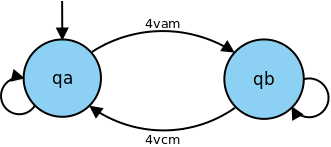
\includegraphics[width=200px,keepaspectratio]{files/VILMA_TRANSITION_EXAMPLE}
	\caption{Exemplo de uma especificação, $4_{vam}$: Transição do estado \textit{Ready} para \textit{Working} no módulo \textit{Vehicle Actuation}, $4_{vcm}$: Transição do estado \textit{Ready} para \textit{Working} no módulo \textit{Vehicle Control}.}
	\label{fig:VILMA_TRANSITION_EXAMPLE}
\end{figure}


Um controle supervisório que garanta o comportamento dos módulos, como um todo, satisfaça a especificação imposta por $S_{i}$ pode ser obtido, dentre outras formas, pelo algoritmo chamado SUPCON ..cite{wonham1987supremal}. Este algoritmo gera sequencias de eventos sob a forma de outro automato $V$, exemplo, $ V = SUPCON(G,S_{i})$, que possa ser implementado para garantir o comportamento do veículo.

Ao expressar vários requisitos sobre o comportamento do veículo em especificações, é possível obter um método sofisticado de controle pode ser desenvolvido que quando implementado pleo SCM vai garantir que o comportamento do veículo atenderá todos os requisitos impostos pelos módulos. Essa abordagem formal permite o desenvolvimento sistemático de estratégias de controle supervisório corretas. Além de permitir a introdução de "inteligencia programada" sobe o comportamento do veículo, consequentemente, melhorando seu grau de autonomia.

% -------------------- NEW SECTION -------------------- 
% -------------------- NEW SECTION -------------------- 
% -------------------- NEW SECTION -------------------- 
\section{Conclusion}\label{chap:conclusion}
% -------------------- NEW SECTION -------------------- 
% -------------------- NEW SECTION -------------------- 
% -------------------- NEW SECTION -------------------- 
% use section* for acknowledgment
\subsection*{Acknowledgment}\label{sec:acknowledgment}
The authors would like to thank...
% trigger a \newpage just before the given reference
% number - used to balance the columns on the last page
% adjust value as needed - may need to be readjusted if
% the document is modified later
%\IEEEtriggeratref{8}
% The "triggered" command can be changed if desired:
%\IEEEtriggercmd{\enlargethispage{-5in}}
% references section
% -------------------- NEW SECTION -------------------- 
% -------------------- NEW SECTION -------------------- 
% -------------------- NEW SECTION -------------------- 
\bibliographystyle{IEEEtran}
\bibliography{references}

% that's all folks
\end{document}